%!TEX root = paper.tex
%%%%%%%%%%%%%%%%%%%%%%%%%%%%%%%%%%%%%%%%%%%%%%%%%%%%%%%%%%%%%%%%%%%%%%%%%%%%%%%%
\section{Evaluation}
\label{sec:eval}

This section presents the results of the online survey
(\S~\ref{subsec:survey}) and
investigates the properties of the actual games offered on the
various platforms (\S~\ref{subsec:platformproperties}).
The survey covers context influence factors including social,
novelty and service-related ones. The platform study scrutinizes
service aspects.

\subsection{Online Survey Results}\label{subsec:survey}
The online survey was completed by $488$ participants
(\SI{91}{\percent} self-identified as male, \SI{8}{\percent} as female), reporting
ages between $13$ and $70$ years (quartiles $21$, $26$, $32$; mode $31$).
All responses were logged in a time frame of four days in early 2018.

\subsubsection{Gaming Demographics}
Around \SI{85}{\percent} of
participants started playing video games before they were ten years old.
Over \SI{50}{\percent} of participants play for $1$--$3$ hours per day.
\SI{44}{\percent} and \SI{36}{\percent} spend \$ $0$--$20$ and \$ $21$--$50$ on games per month, respectively.
Almost 50\% of participants own between $101$ and $500$ games, and about
15\% report to own $11$ to $50$ and $501$ to $1000$ games, respectively.
More than 40\% of participants bought $3$ to $10$ games in the last
twelve months; slightly more than 45\% claim to have bought
$10$ to $100$ games.



\subsubsection{Social Context Factors And Novelty}

When asked to mark all ways of learning about new games, respondents
most prevalently selected ``news on gaming sites'', ``reviews'', and
``friends'' (about \SI{60}{\percent} each). Other popular factors include
``live streams'', ``recommendations in online stores'', and
``gaming bundles'' (with \SI{40}{\percent}, \SI{30}{\percent}, and \SI{20}{\percent} each). Retail stores are hardly mentioned.
The popularity of games on \textit{Twitch} (a website dedicated to
live streaming of video games) or with game critics is judged as not
important to over \SI{70}{\percent} and over \SI{60}{\percent} of participants, respectively.

\subsubsection{System Influence Factors}
Almost all participants (\SI{97}{\percent}) own a PC, the two other most prevalent
gaming systems are smartphones (\SI{30}{\percent}) and Sony's PlayStation 4 (\SI{26}{\percent}).
Nintendo's Switch and 3DS as well as Microsoft's XBox One are reported
by between \SI{18}{\percent} and \SI{11}{\percent} of participants.
\SI{93}{\percent} report the PC to be their favorite gaming system, with consoles
favored by \SI{29}{\percent}.



\subsubsection{Service Factors}

Digital gaming stores (and among these, \steam) are reported as
the most popular ways of obtaining games. About \SI{85}{\percent} of respondents
use digital storefronts. The other proposed selections reach far lower
values: ``third-party key sellers'' hits \SI{35}{\percent}, and both ``physical
games from online stores'' and ``physical games from retailers''
are capped around \SI{25}{\percent}.
90\% of participants use the \steam platform; \textit{Humble Bundle}
and \textit{GOG} are very popular (almost \SI{60}{\percent}) as well. \textit{Origin}
at \SI{38}{\percent} is a relatively distant fourth already. None of the other
proposed selections, including the console-specific digital stores
(PlayStation Network/Store, Nintendo eShop, XBox Store), exceed
\SI{25}{\percent}.

Figure~\ref{fig:buying-factors} shows the respondents' assessments
of factors important for buying new gaming systems, grouped by
importance. As can be seen, system prices are a motivator for
almost \SI{70}{\percent} of survey participants. Online multiplayer capabilities,
system-exclusive games, and graphics are important or very important
for more than \SI{40}{\percent}, each. On the other side, local multiplayer
capabilities, the mere recency of games, and available downloadable
content are deemed relatively unimportant factors for a buying decision.

The survey also asked about buying hindrances for newly released 
games, i.e. reasons that speak against buying them.
More than \SI{70}{\percent} of participants declare a lack of interest
that hinders them. Financial reasons play a role for roughly
a third of respondents, and a similar proportion has a substantial
backlog of games awaiting to be played, whereas only \SI{15}{\percent} declared
their hardware to be lacking support for the latest games.


\begin{figure}[!t]
	\centering
	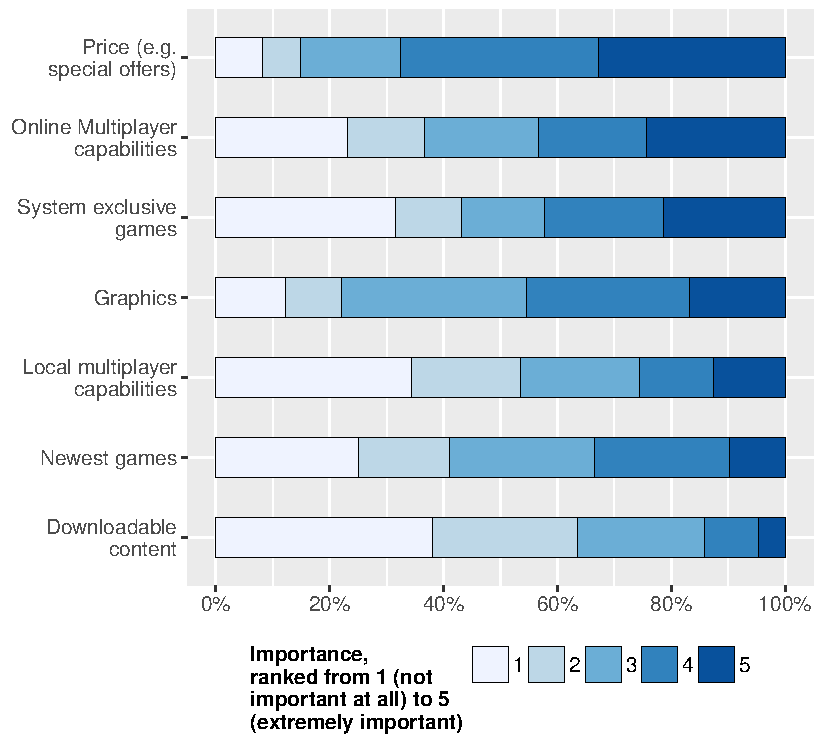
\includegraphics[width=1.0\columnwidth]{images/buyingfactors.pdf}
	\caption{Respondents' assessment of factors important for buying
	new gaming systems.}
\label{fig:buying-factors}
\end{figure}


\subsection{Game Platform Properties}\label{subsec:platformproperties}

To complement the subjective gamer results and also provide an
inter-platform comparison, the attention now turns to the service
factors of three gaming platforms: \steam, \gfnow, and \psnow.
Table~\ref{tab:game-stats} provides an overview of the data
collected, showing the number, age, length, and review scores
across platforms.

%%%%%%%%%%%%

\begin{table*}
\centering
\caption{Game characteristics on the investigated platforms. Title counts from Web/API scraping, lengths from \hltb, ages and review scores from \metacritic.}
\label{tab:game-stats}
	\begin{tabu}{X[2]|X[r]X[r]X[r]X[r]X[r]X[r]X[r]}
	\toprule
	Service & Titles & Age $\mu$ & Age $\sigma$ & Length $\mu$ & Length $\sigma$ & Score $\mu$ & Score $\sigma$ \\
	\midrule
	\gfnow & $118$ & \SI{3.1}{\year} & \SI{\pm2.3}{\year} & \SI{10.7}{\hour} & \SI{\pm8.2}{\hour} & $73.9$ & $\pm10.1$ \\
	\psnow & $432$ & \SI{4.8}{\year} & \SI{\pm2.4}{\year} & \SI{8.8}{\hour} & \SI{\pm8.8}{\hour} & $71.9$ & $\pm12.0$ \\
	\steam & $14,120$ & \SI{2.5}{\year} & \SI{\pm3.3}{\year} & \SI{7.3}{\hour} & \SI{\pm10.2}{\hour} & $70.6$ & $\pm11.0$ \\
	\bottomrule
	\end{tabu}
\end{table*}


%%%%%%%%%%%%
\subsubsection{Number of Games}

The two cloud
platforms offer a very limited number of games when compared to the
games available on \steam, which itself again only represents a subset
of all games available either on the PC platform (\metacritic lists
\num{26420}) or across all platforms (\num{57308}). Two
possible, simple explanations for the low game count on the cloud
platforms come to mind: One is that they were launched relatively
recently (2015) in comparison to \steam (2003), leaving little time for
the range of games to grow. Secondly, the choice of games for a cloud
gaming platform is most likely curated by the platform operator for
compatibility and performance reasons. This usability burden shifts to
the end user for digital storefronts like \steam, allowing these
platforms to offer a larger variety of games, including ones that are
very demanding on the hardware.


%%%%%%%%%%%%
\subsubsection{Game Ages}

The average
game ages appear to be relatively high for all of the investigated
platforms, and particularly so for \psnow. It might be considered a
special case, as it is specifically advertised as a backwards
compatibility for older, pre-PlayStation 4 games that do not run on the
latest Sony platform any more. For \steam, the distribution is
significantly skewed towards recent titles: A quarter of games are less
than a year old, and the median is at $21$ months. The
distribution's tail extends beyond $25$ years due to re-releases
of ``classic'' games on the platform.


%%%%%%%%%%%%
\subsubsection{Game Lengths}
Figure~\ref{fig:gamelengths-violin} shows the distribution of aggregated
game lengths for the three platforms under investigation, and an
``overall'' distribution that includes further platforms and gaming
systems. Among the three platforms, the median reported game
length is largest for \gfnow. In
contrast to the curated choice of games on the Cloud systems, \steam
also offers shorter and longer games.

\begin{figure}[!t]
	\centering
	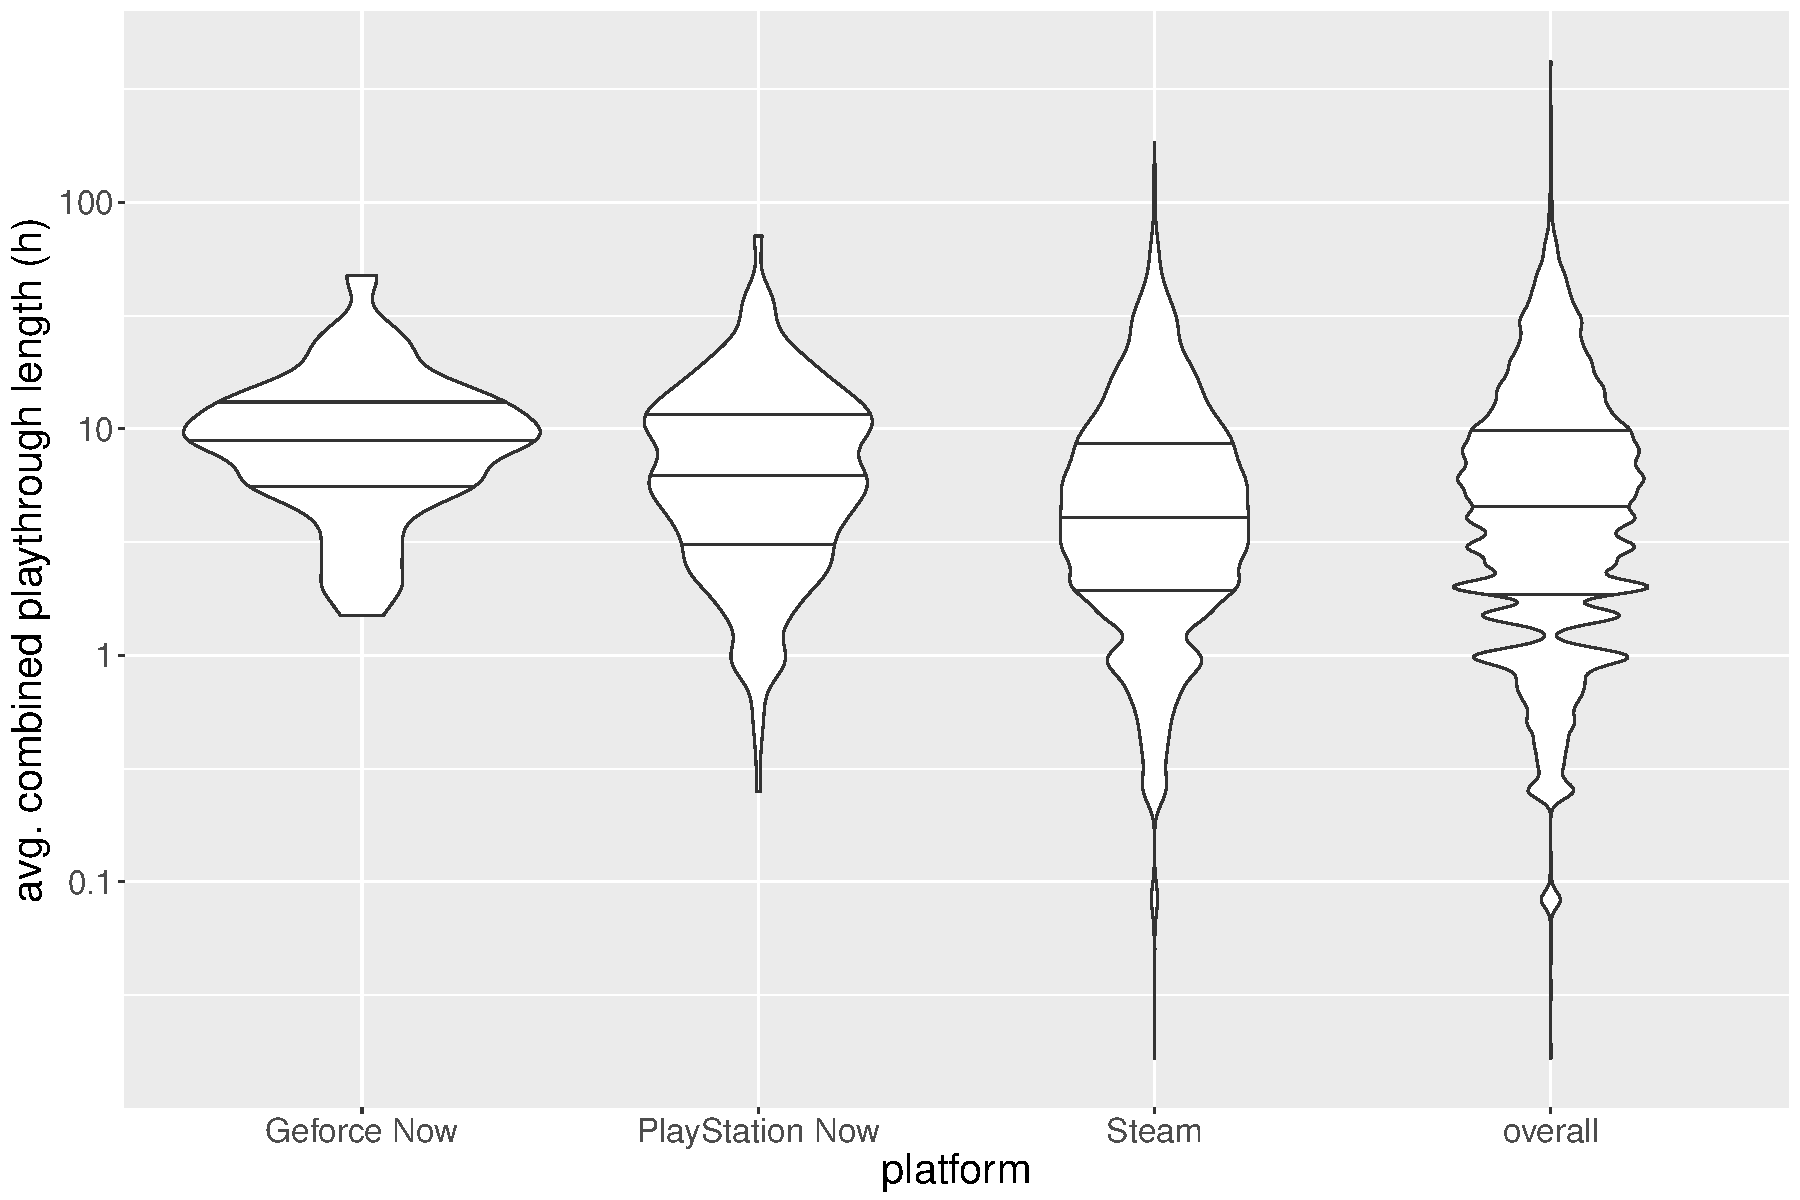
\includegraphics[width=1.0\columnwidth]{images/gamelengths-by-platform-violin.pdf}
	\caption{Violin plot of the per-platform average game lengths from \hltb. Quartiles indicated by horizontal lines.}
\label{fig:gamelengths-violin}
\end{figure}


%%%%%%%%%%%%
\subsubsection{Game Prices}

Trying to compare the prices per game is a difficult endeavor, due to
the mixed approach of the gaming platforms. The \gfnow subscription
gives customers access to a subset of its catalog that can be
extended by purchasing additional games; \gfnowpc 
on the other hand requires the customer to buy games on their
own and pay for the time spent playing.
\psnow and \psnowpc have a flat rate for all of their catalog.
At least for \steam, unit prices can be discussed.
Between mid-2015 when the authors started monitoring \steam's catalog,
and late 2017 when the last measurement was taken,
its average price has decreased from \SI{10.11}[\$]{} to \SI{8.83}[\$]{}. In the same
timeframe, the number of games more than doubled, from \num{5996} to
\num{14120}. The prices vary a lot over time, for instance due to
seasonal sales periods.

\begin{figure}[!t]
	\centering
	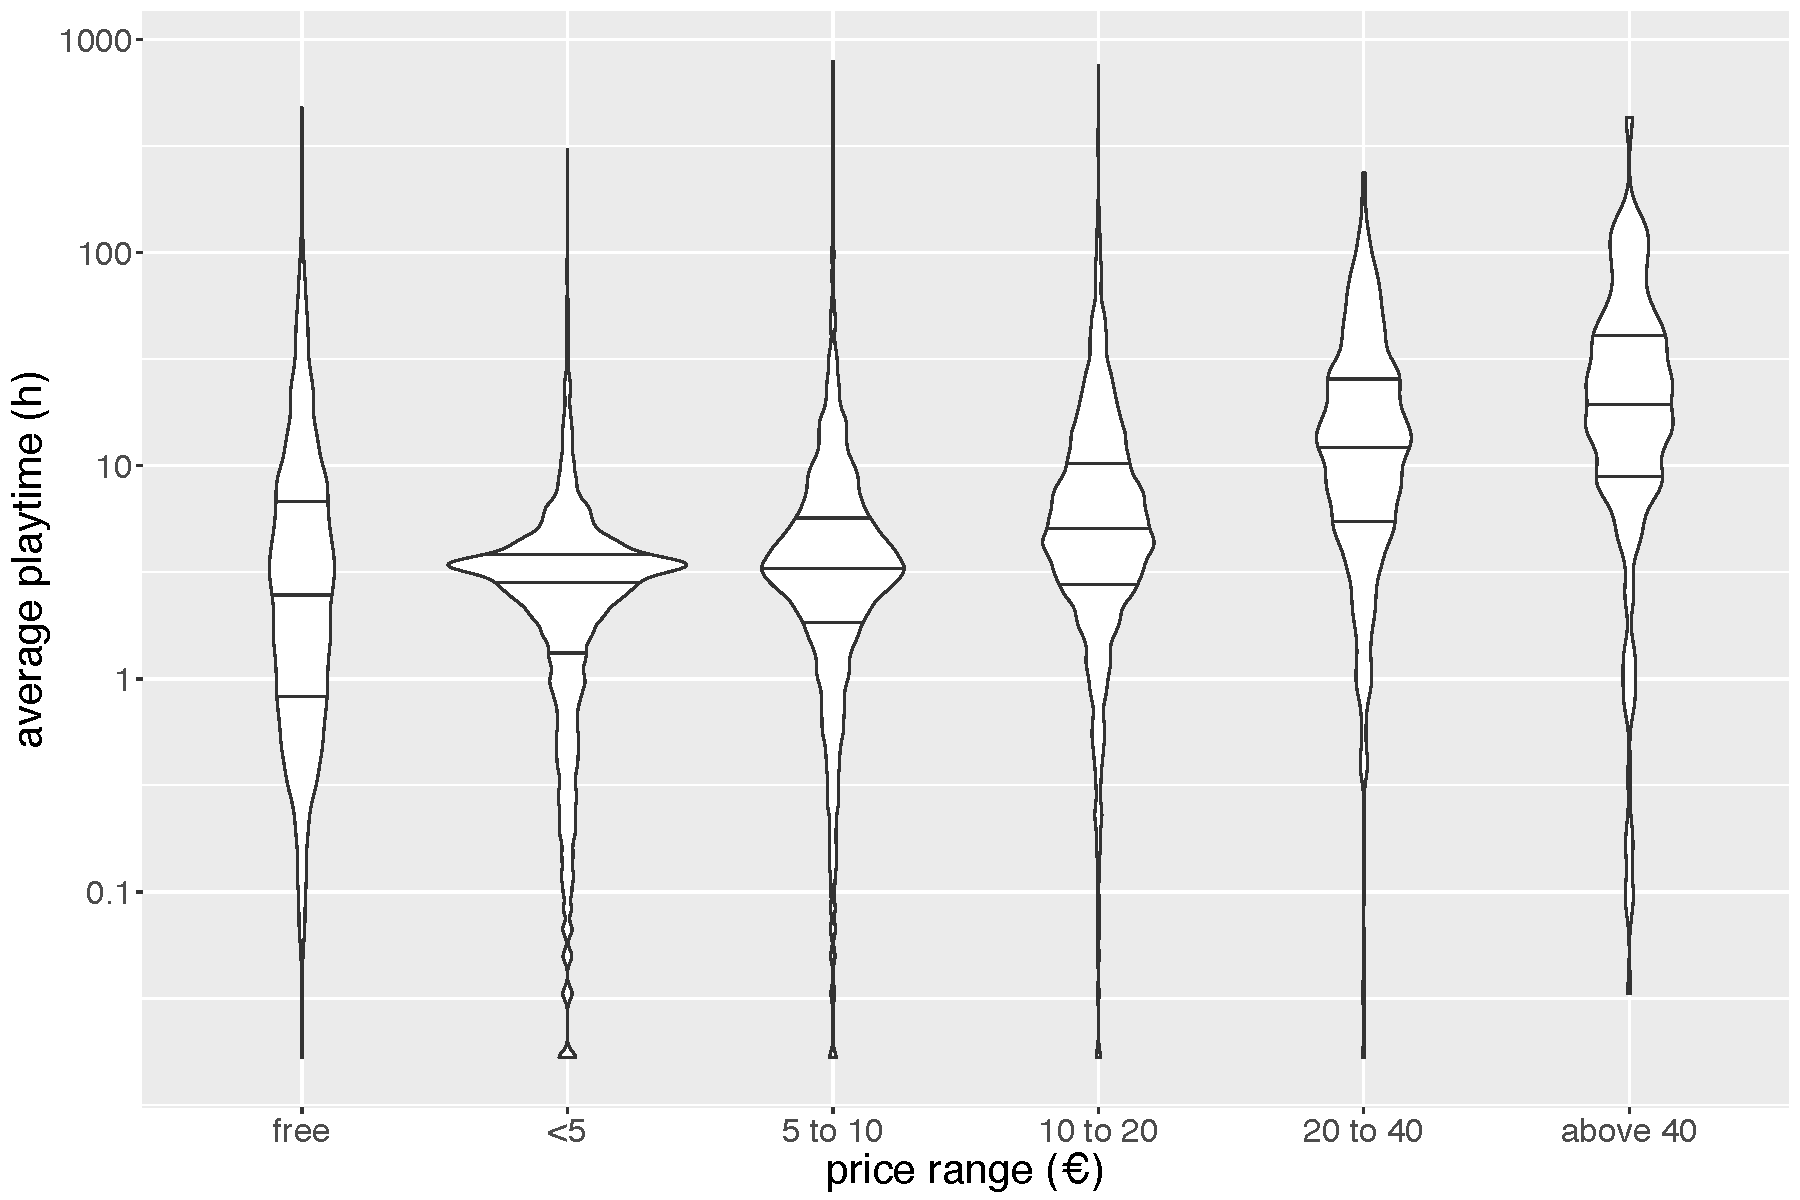
\includegraphics[width=1.0\columnwidth]{images/steam-cost-vs-playtime-non-sale.pdf}
	\caption{Violin plot of the average playtime of \steam games, broadly categorized by their price ranges. The number of games per bin are $1541$, $5269$, $4019$, $2445$, $658$, and $188$. Quartiles indicated by horizontal lines.}
\label{fig:steam-cost-vs-playtime-violin}
\end{figure}

\subsubsection{Price versus Playtime}
Again focusing on \steam,
Figure~\ref{fig:steam-cost-vs-playtime-violin} breaks down the
distribution of average playtimes per game price range. The game price
ranges are chosen so as to roughly separate the prevalent modes of the
price distribution.
Playtime is defined as the time game owners spend playing a game, as
recorded by the \steam platform and scraped from \textit{SteamSpy}.
Playtimes of ``free'' titles 
span almost the whole playtime range.
For games that cost less than \SI{5}[\EUR]{}, the mode is around
\SI{3.5}{\hour} of playtime, and values are concentrated around it.
This recent trend only
manifested itself in datasets in the last twelve months: 
The number of games in this price category grew by a factor of
$2.4$ in that timeframe, whereas they
increased by only \SI{37}{\percent} in the free price range, and roughly doubled
in the other price ranges.

Other than that, the median playtime increases with the price range;
unfortunately, the data does not explain the cause: E.g., more expensive
games might have more playable content, causing the playtime to
increase. Conversely, higher upfront costs may incite players to spend
more time regardless of game quality, thus avoiding regret for the
expense.


%%%%%%%%%%%%
\subsubsection{Review Scores}

The final characteristic presented from the data are game review scores as
given by professional gaming media outlets. This relies on the
\metacritic dataset. This set covers review scores for all current
and historic gaming platforms. The review scores are aggregated to
average scores ranging between $0$ and $100$. Some \metacritic-internal
weighing factors are applied to express the importance of some media
outlets over others.
The average scores exceed $70$ across all services, albeit with a
slightly lower $\sigma$ for \gfnow.



\subsection{Subjective Assessments Of Utility Metrics}

Finally, the survey also included questions that directly target
the utility metrics of platforms described above.
To put prices and playtimes into perspective, the survey asked
whether $5$ to $10$ hours of gameplay were enough for a price of \SI{60}[\$]{}.
More than \SI{50}\% of participants strongly disagreed, and more than
\SI{20}{\percent} disagreed. This demand-side rejection clearly fits the picture of
Figure~\ref{fig:steam-cost-vs-playtime-violin}, where less than a
quarter of games that cost more than \SI{40}[\EUR]{} are played for less than
$10$ hours.

The absence of game recency as a motivational factor was discussed
above already; other motivational factors that respondents strongly
agreed to were preferences of gameplay over graphics, and gaming
experience in general (both reaching almost \SI{80}{\percent} importance ratings).
Also, over half of the respondents value replayability, i.e. to
be able to play a game more than once.

A result relevant for the curated offers of \gls{cg}
platforms is that almost \SI{80}{\percent} or respondents are not interested in
exchanging flat-rate access fees for buying individual games.
Other responses from survey participants indicate a multitude of
interests and motivations for and against platforms, including
statements like ``I buy only games with Linux support'',
or hints at the availability of ``pirated'' games.
